\hypertarget{BasicPlayer_8cpp}{}\section{src/\+Basic\+Player.cpp File Reference}
\label{BasicPlayer_8cpp}\index{src/\+Basic\+Player.\+cpp@{src/\+Basic\+Player.\+cpp}}
{\ttfamily \#include \char`\"{}Basic\+Player.\+h\char`\"{}}\\*
{\ttfamily \#include \char`\"{}Parse.\+h\char`\"{}}\\*
Include dependency graph for Basic\+Player.\+cpp\+:
\nopagebreak
\begin{figure}[H]
\begin{center}
\leavevmode
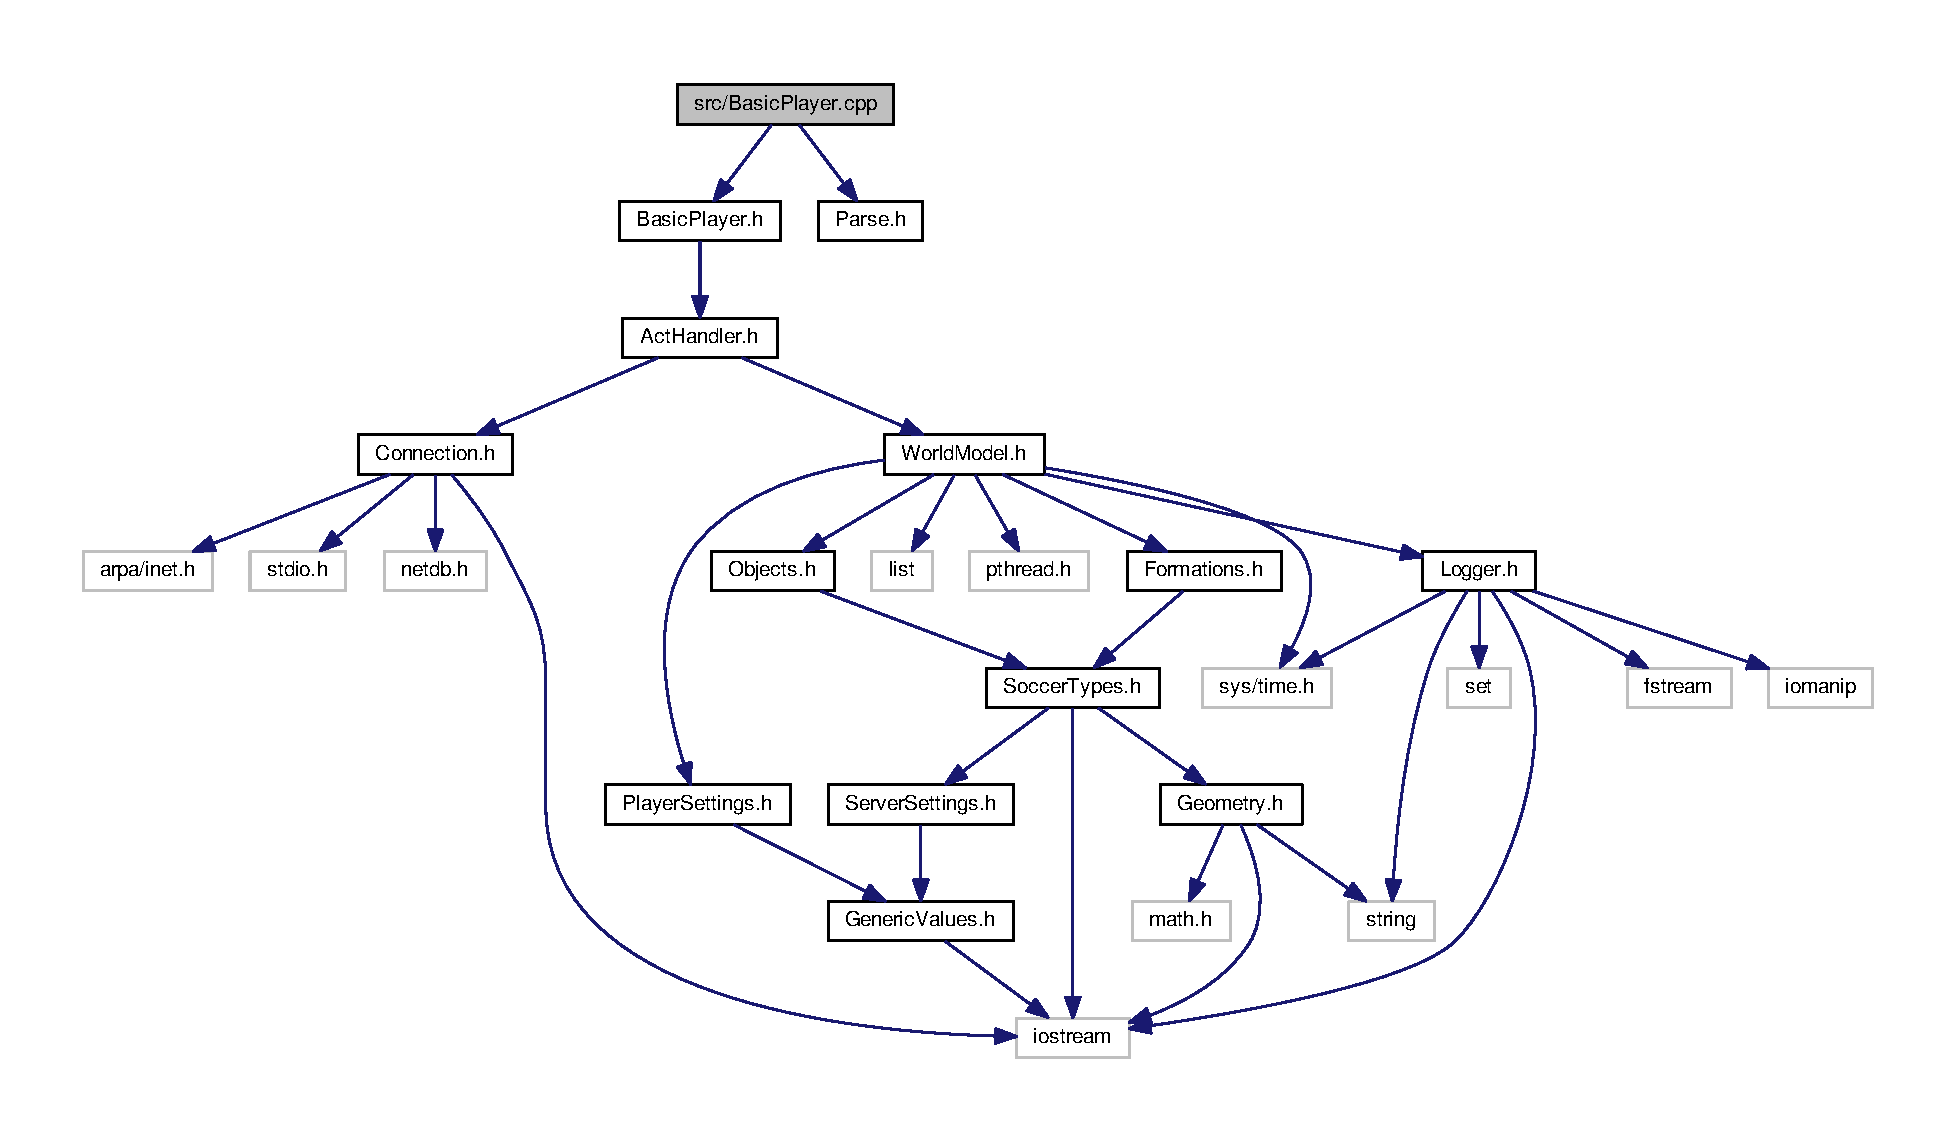
\includegraphics[width=350pt]{BasicPlayer_8cpp__incl}
\end{center}
\end{figure}


\subsection{Detailed Description}

\begin{DoxyPre}
{\bfseries File:}          \hyperlink{BasicPlayer_8cpp}{BasicPlayer.cpp}
{\bfseries Project:}       Robocup Soccer Simulation Team: UvA Trilearn
{\bfseries Authors:}       Jelle Kok
{\bfseries Created:}       10/12/2000
{\bfseries Last Revision:} $ID\$
{\bfseries Contents:}      This file contains the class declaration for the
               \hyperlink{classBasicPlayer}{BasicPlayer}. The \hyperlink{classBasicPlayer}{BasicPlayer} is the class where the
               available skills for the agent are defined.



\subsubsection*{{\bfseries Changes}}\end{DoxyPre}



\begin{DoxyPre}
{\bfseries Date}             {\bfseries Author}          {\bfseries Comment}:
10/12/2000       Jelle Kok       Initial version created
\end{DoxyPre}
 